\subsection{Class diagram di design}
    \begin{flushleft}
        Verranno di seguito riportati i class diagram di design, che ora rispecchiano l'architettura del sistema e tutte le funzionalità nella loro
        interezza. \\
        Si noti che per migliorare la leggibilià i diagrammi sono stati divisi in delle macrocategorie seguendo quelli che erano i modelli di dominio precedenti.
        Ogni diagramma è completo delle funzionalità descritte precedentemente negli use case e nei requisiti.\\
        \emph{\textbf{Nota}}: Tutti i costruttori banali (senza argomenti) e i getter e i setter sono stati omessi per rendere più leggibili i diagrammi.\\
        \emph{\textbf{Nota 2}}: Le componenti grafiche (TextView, Button, ecc.) potrebbero non essere tutte presenti come attributi della classe, in quanto a volte sono stati dichiarati localmente nelle funzioni.
        
    \end{flushleft}

    \subsubsection{Login}
        \begin{figure}[H]
            \centering
            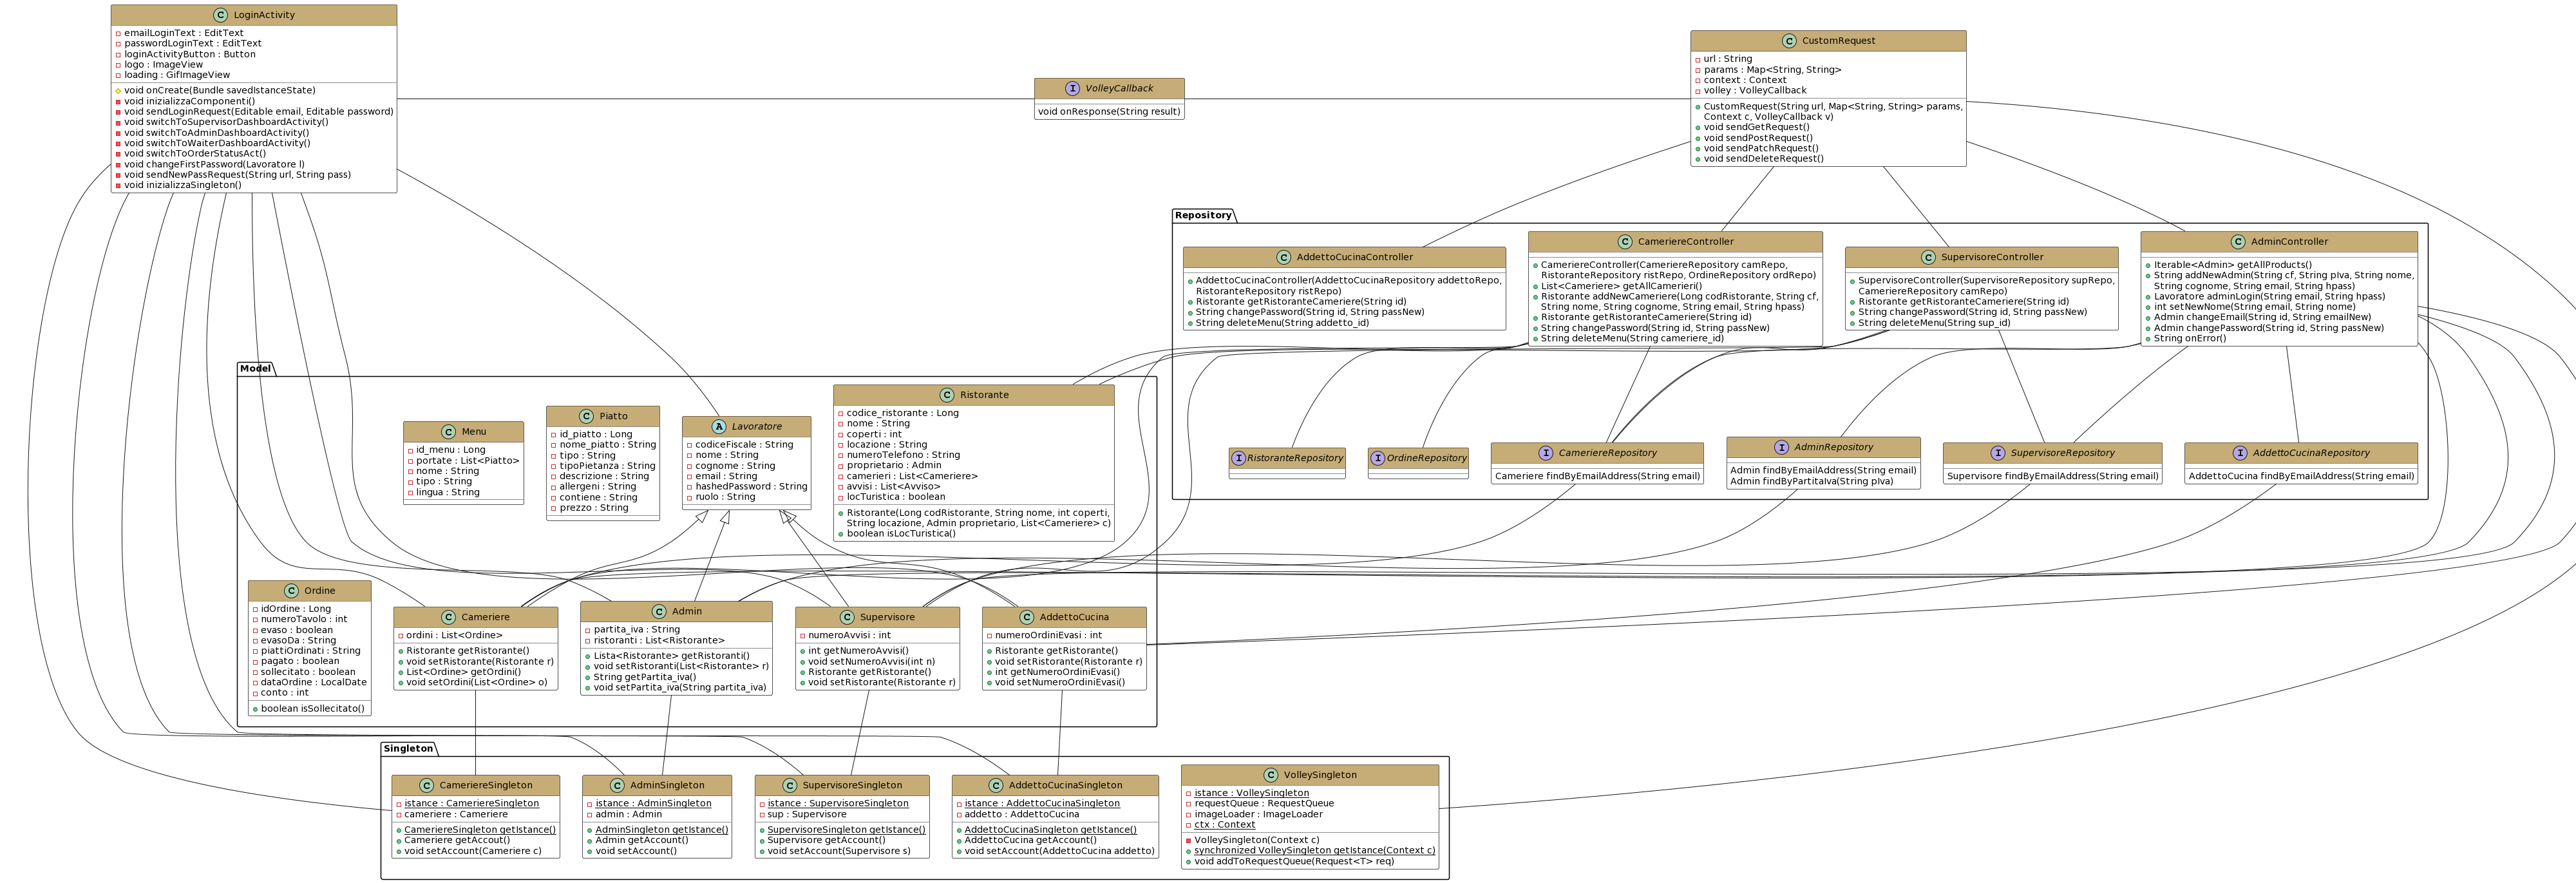
\includegraphics[scale=0.12]{assets/diagrammi/Class diagram di design/ClassDiagram_Login.png}
            \caption*{\textbf{CD01}: Class diagram Login}\label{fig:ClassDiagram_Login}
        \end{figure}
    
    \subsubsection{Gestione piatti}
        \begin{figure}[H]
            \centering
            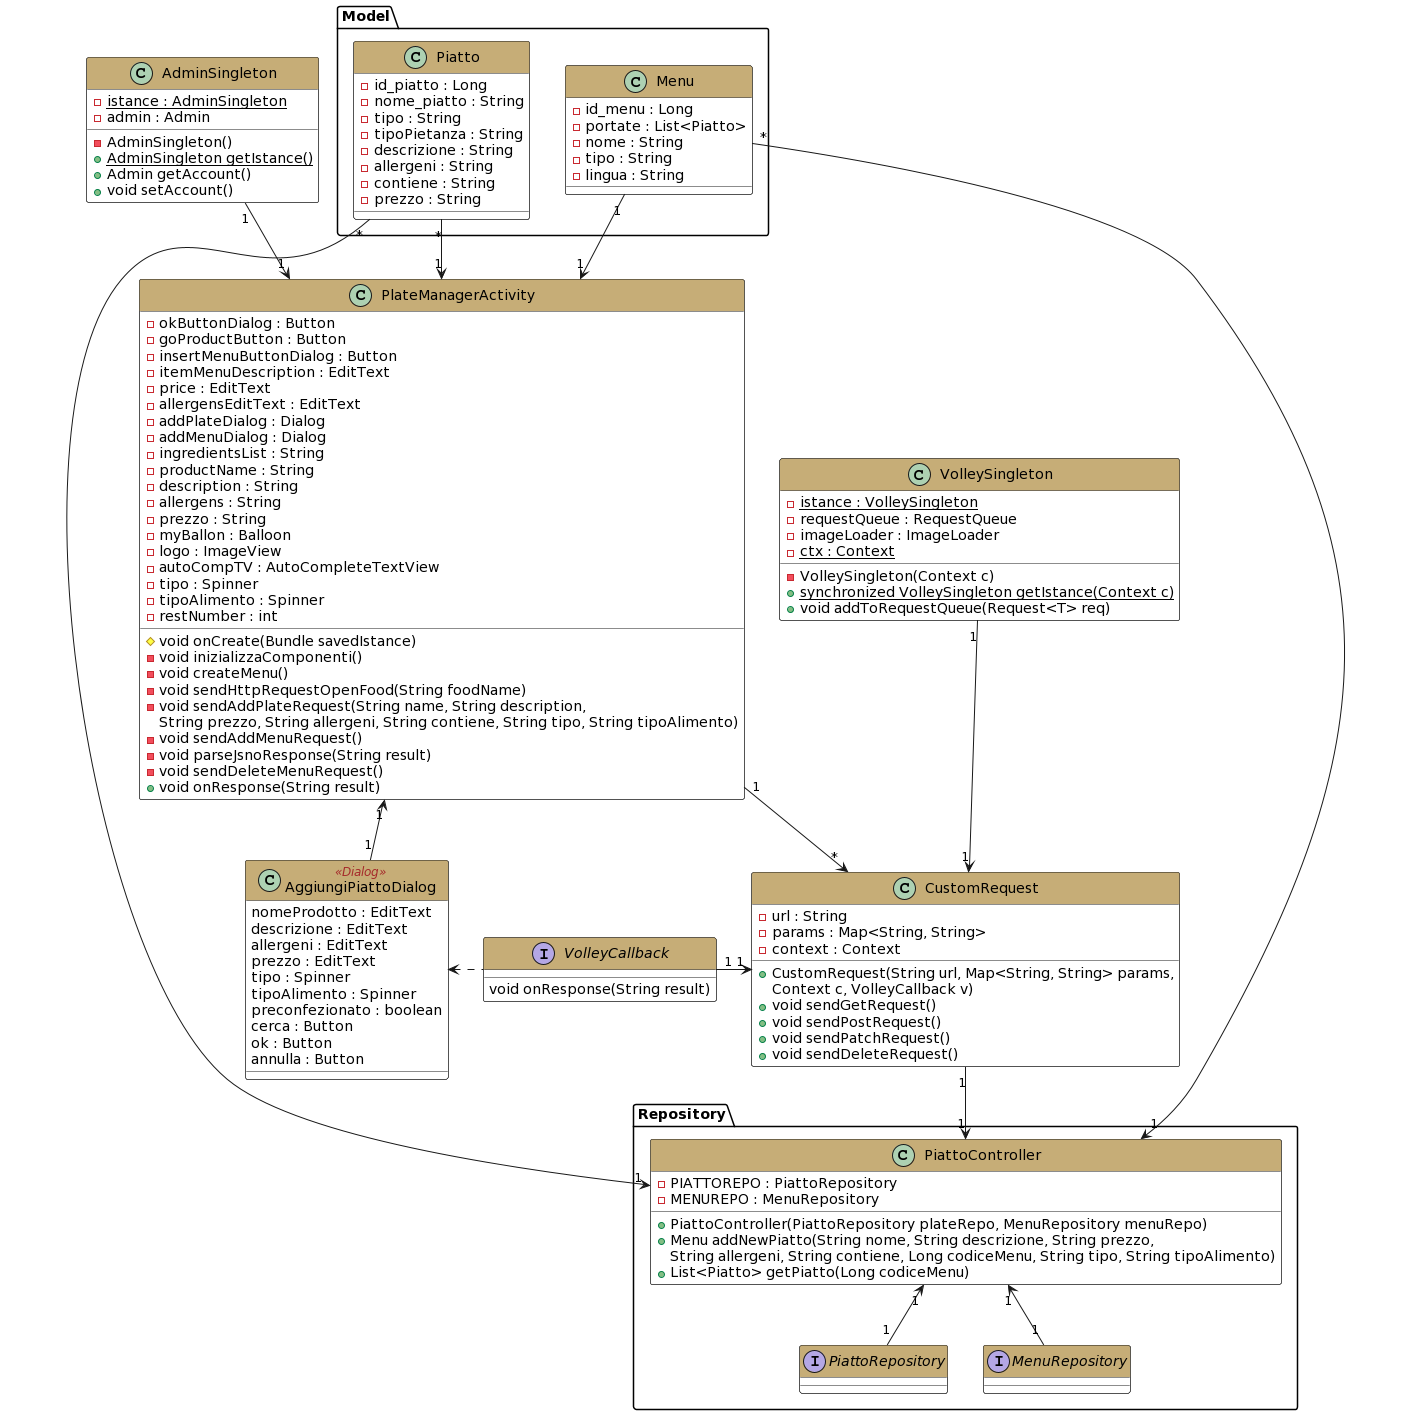
\includegraphics[scale=0.25]{assets/diagrammi/Class diagram di design/gestione piatti.png}
            \caption*{\textbf{CD02}: Class diagram gestione piatti}\label{fig:ClassDiagram_ManagePlates}
        \end{figure}

    \subsubsection{Gestione Avvisi}
        \begin{figure}[H]
            \centering
            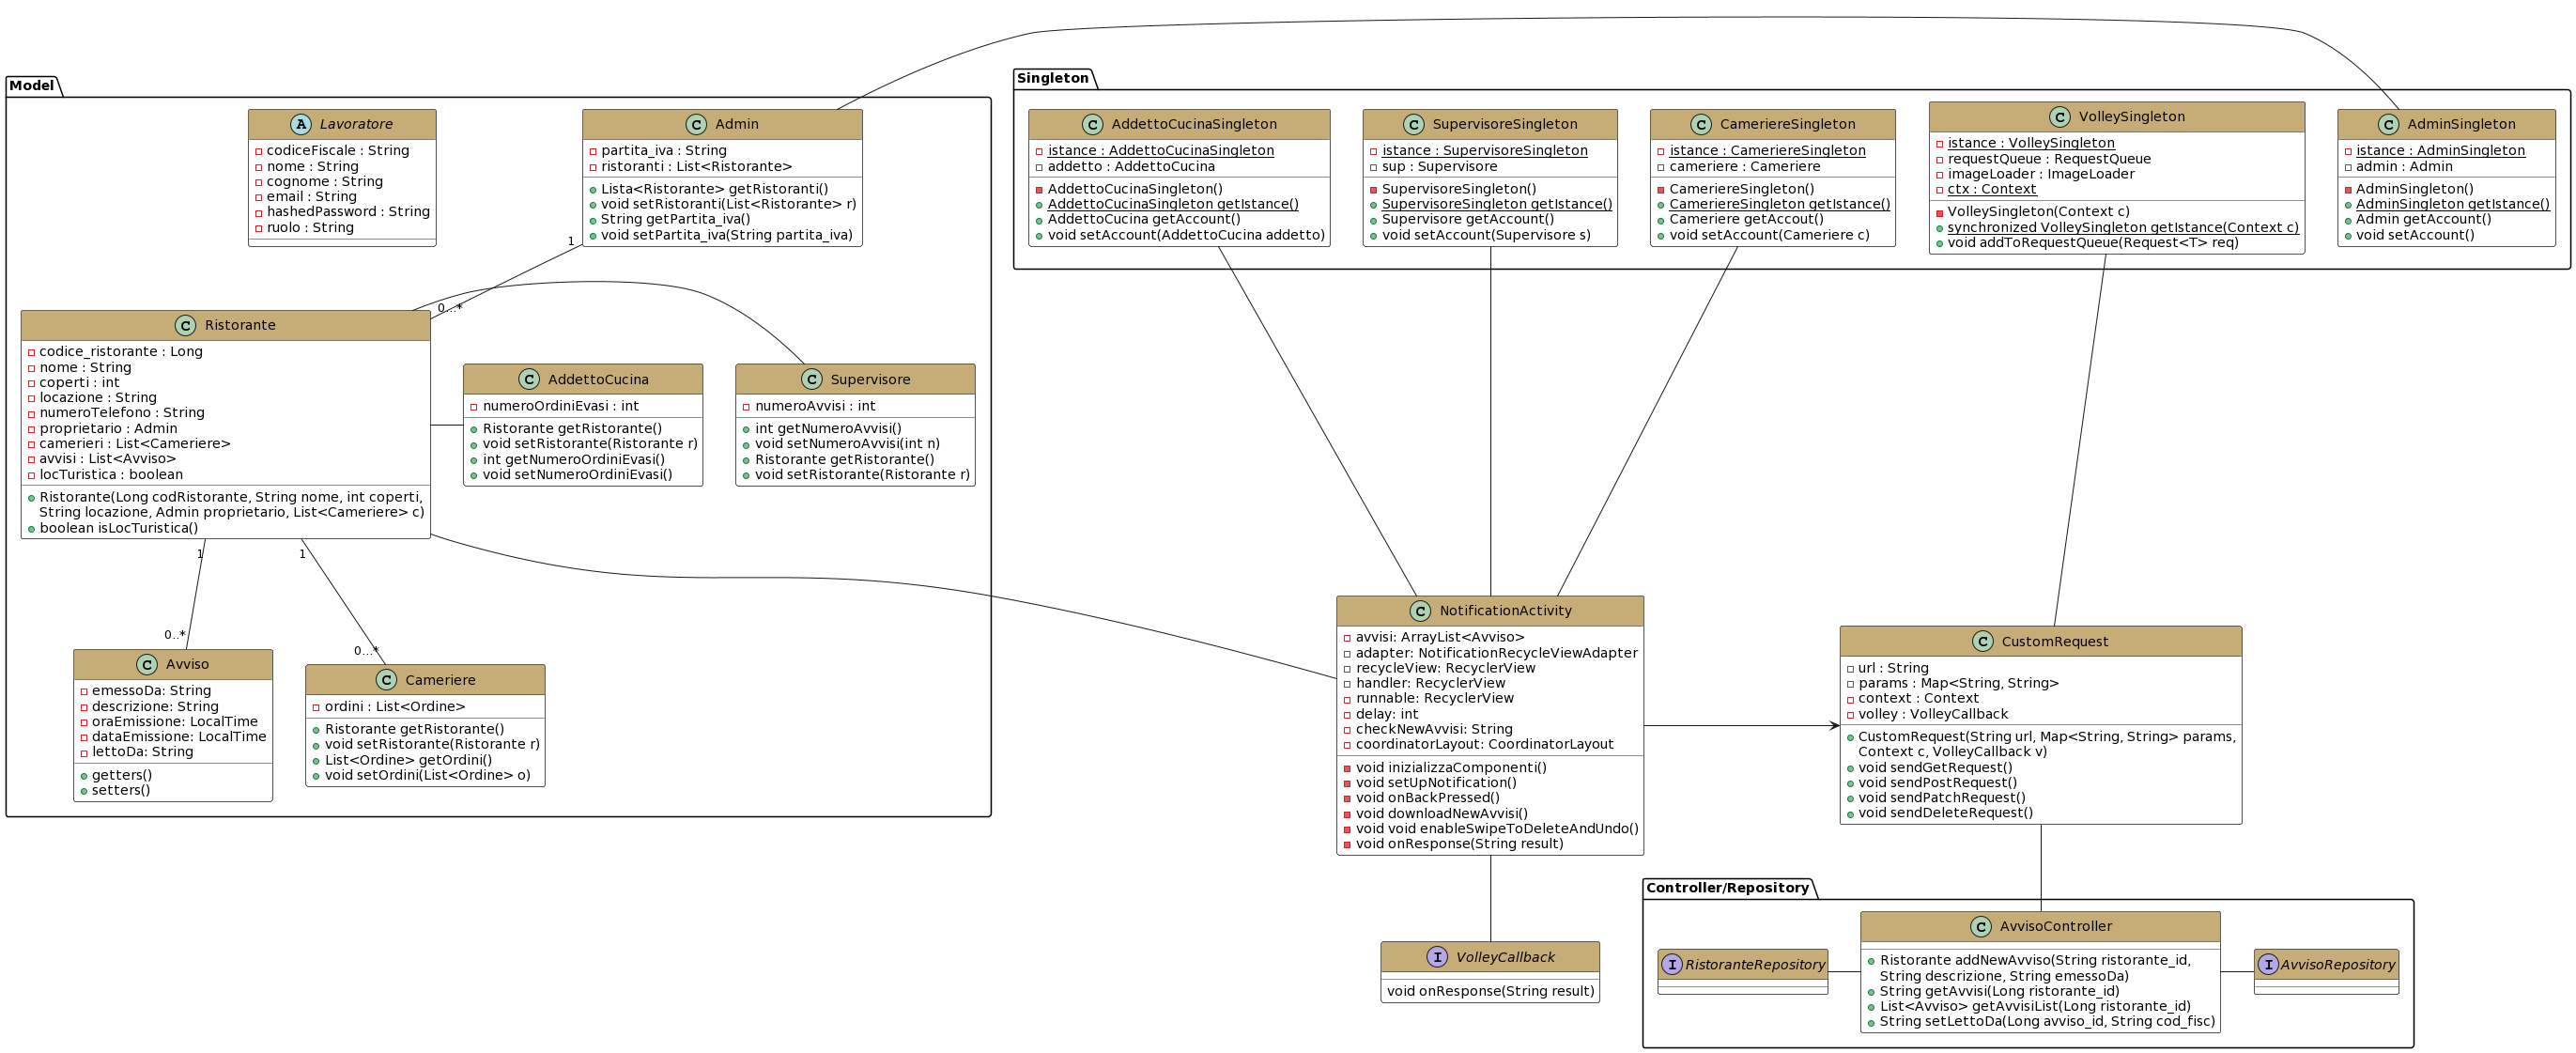
\includegraphics[scale=0.15]{assets/diagrammi/Class diagram di design/ClassDiagramGestioneAvvisi.png}
            \caption*{\textbf{CD03}: Class diagram gestione avvisi}\label{fig:ClassDiagram_ManageAdv}
        \end{figure}

    \subsubsection{Gestione Ordini}
        \begin{figure}[H]
            \centering
            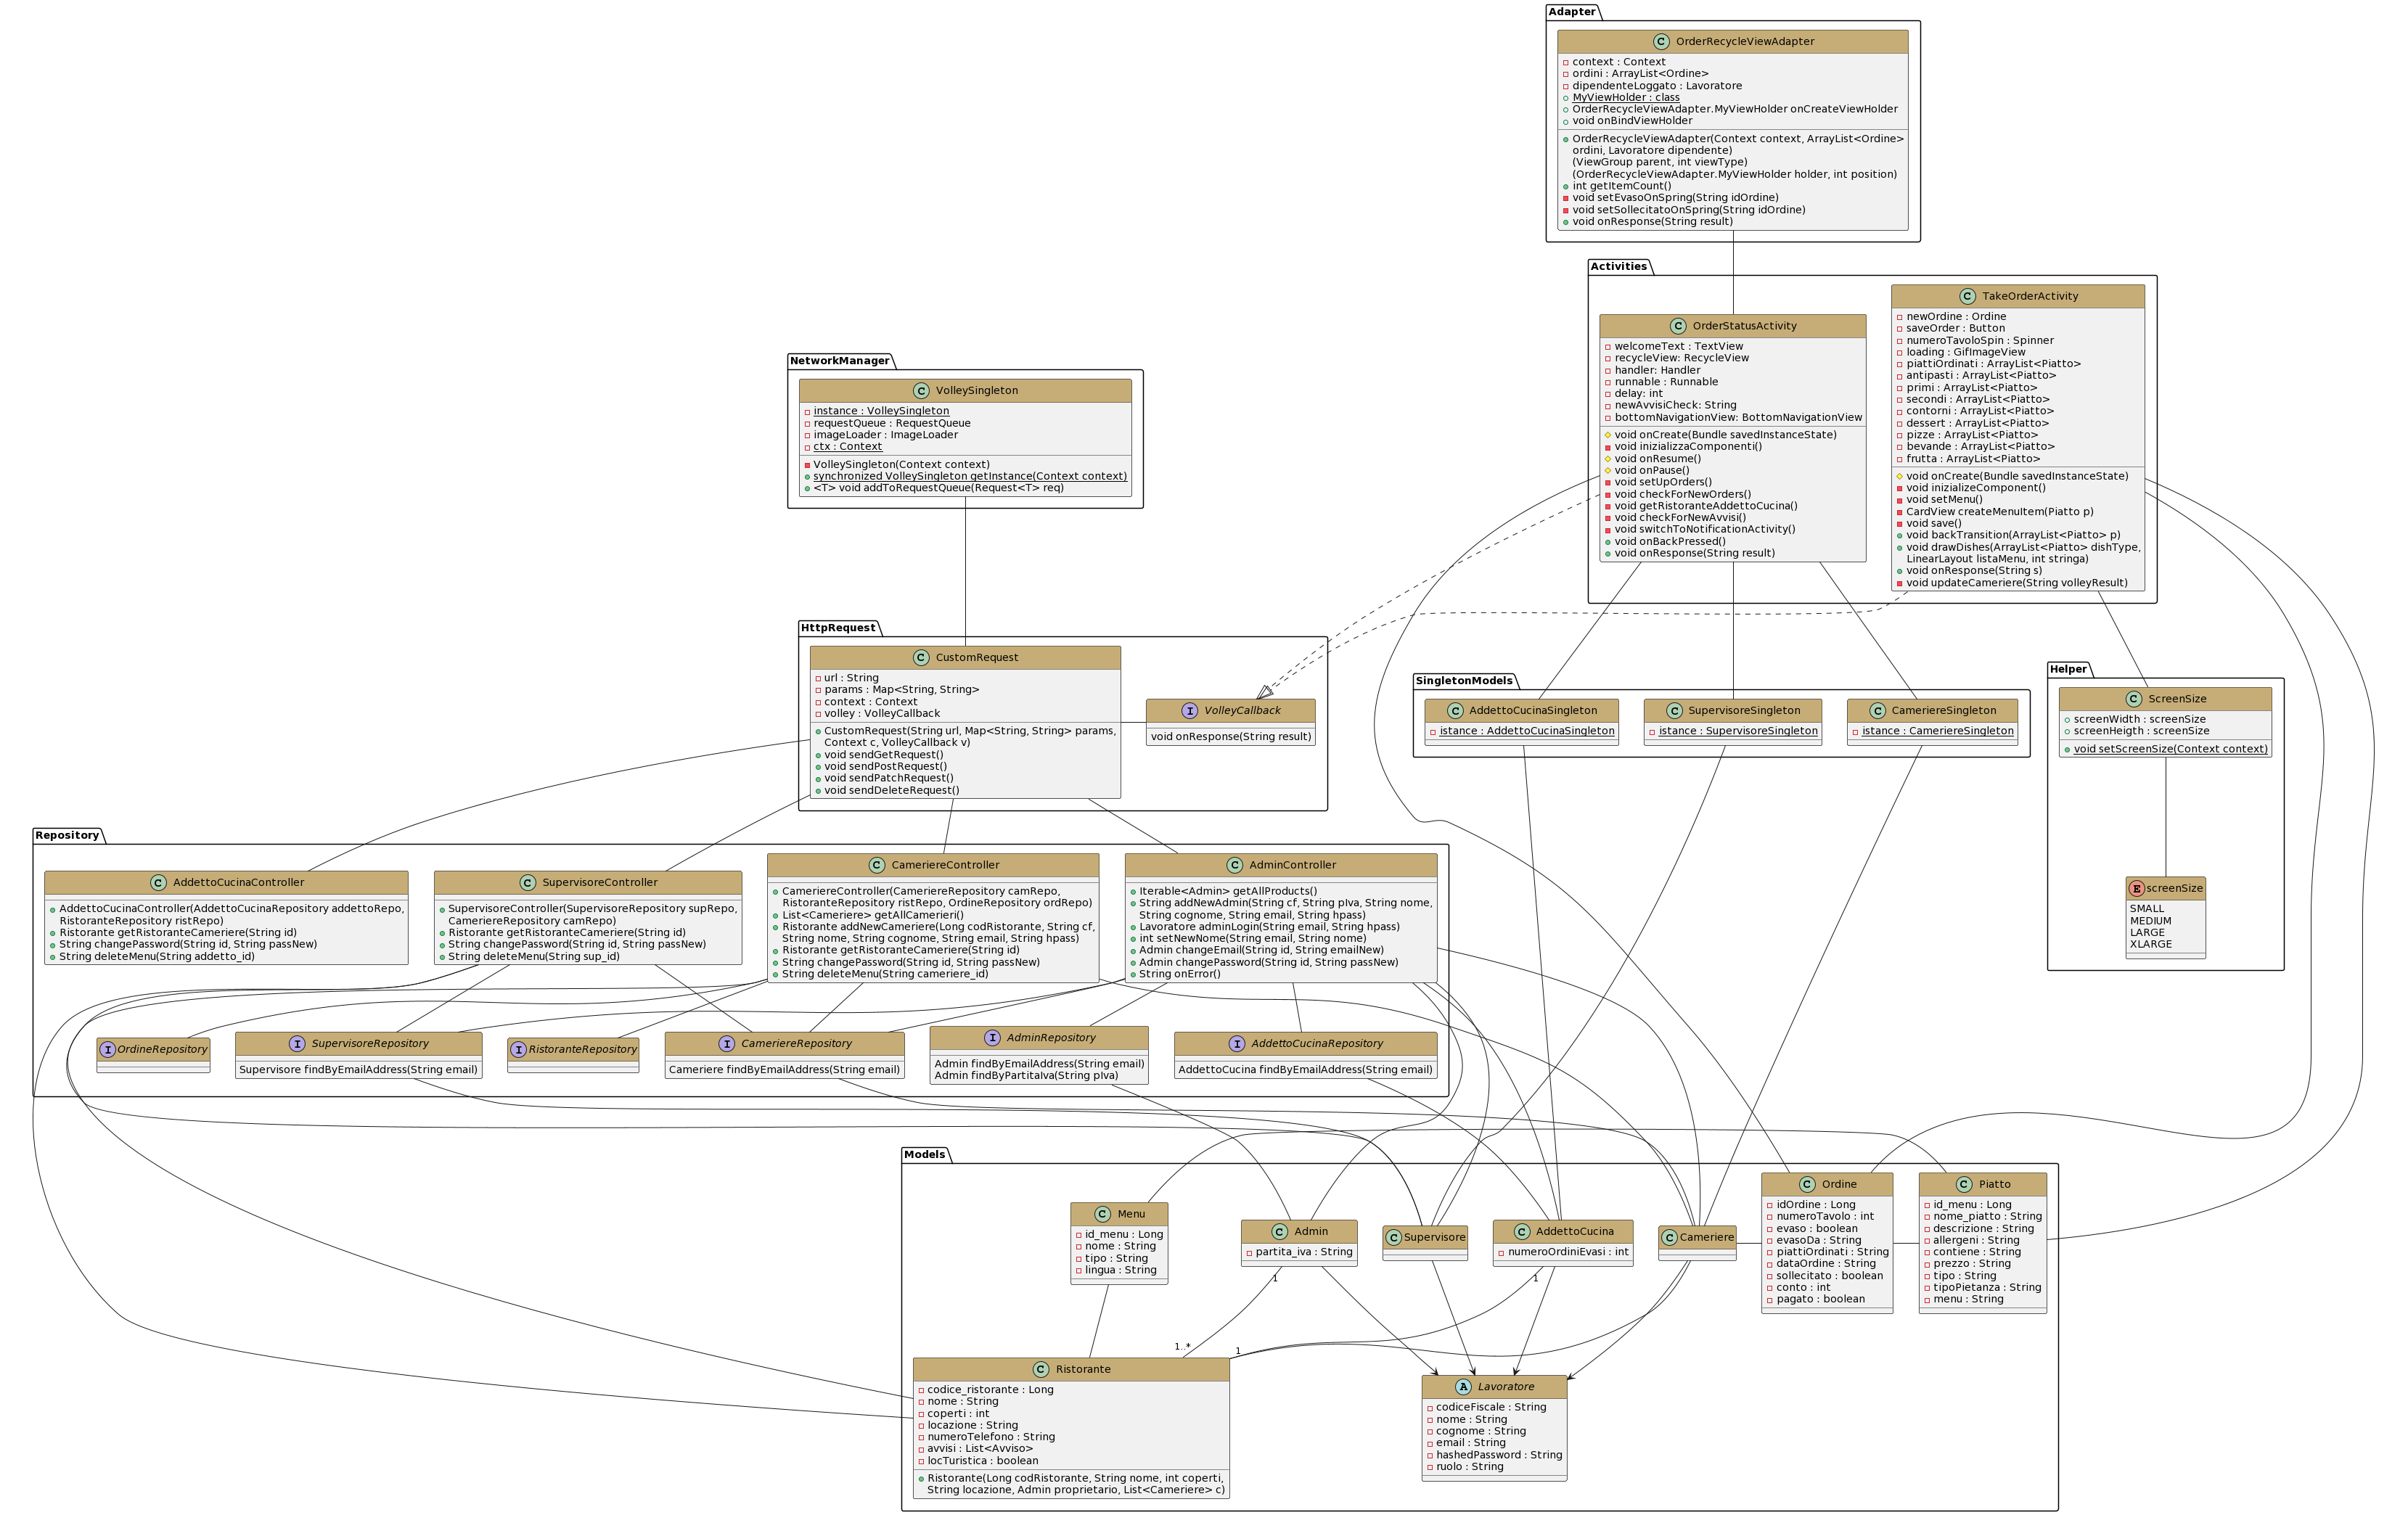
\includegraphics[scale=0.15]{assets/diagrammi/Class diagram di design/Class Diagramm Design Gestione Ordini.png}
            \caption*{\textbf{CD03}: Class diagram gestione ordini}\label{fig:ClassDiagram_ManageOrders}
        \end{figure}

    \subsubsection{Gestione Dipendenti}
        \begin{figure}[H]
            \centering
            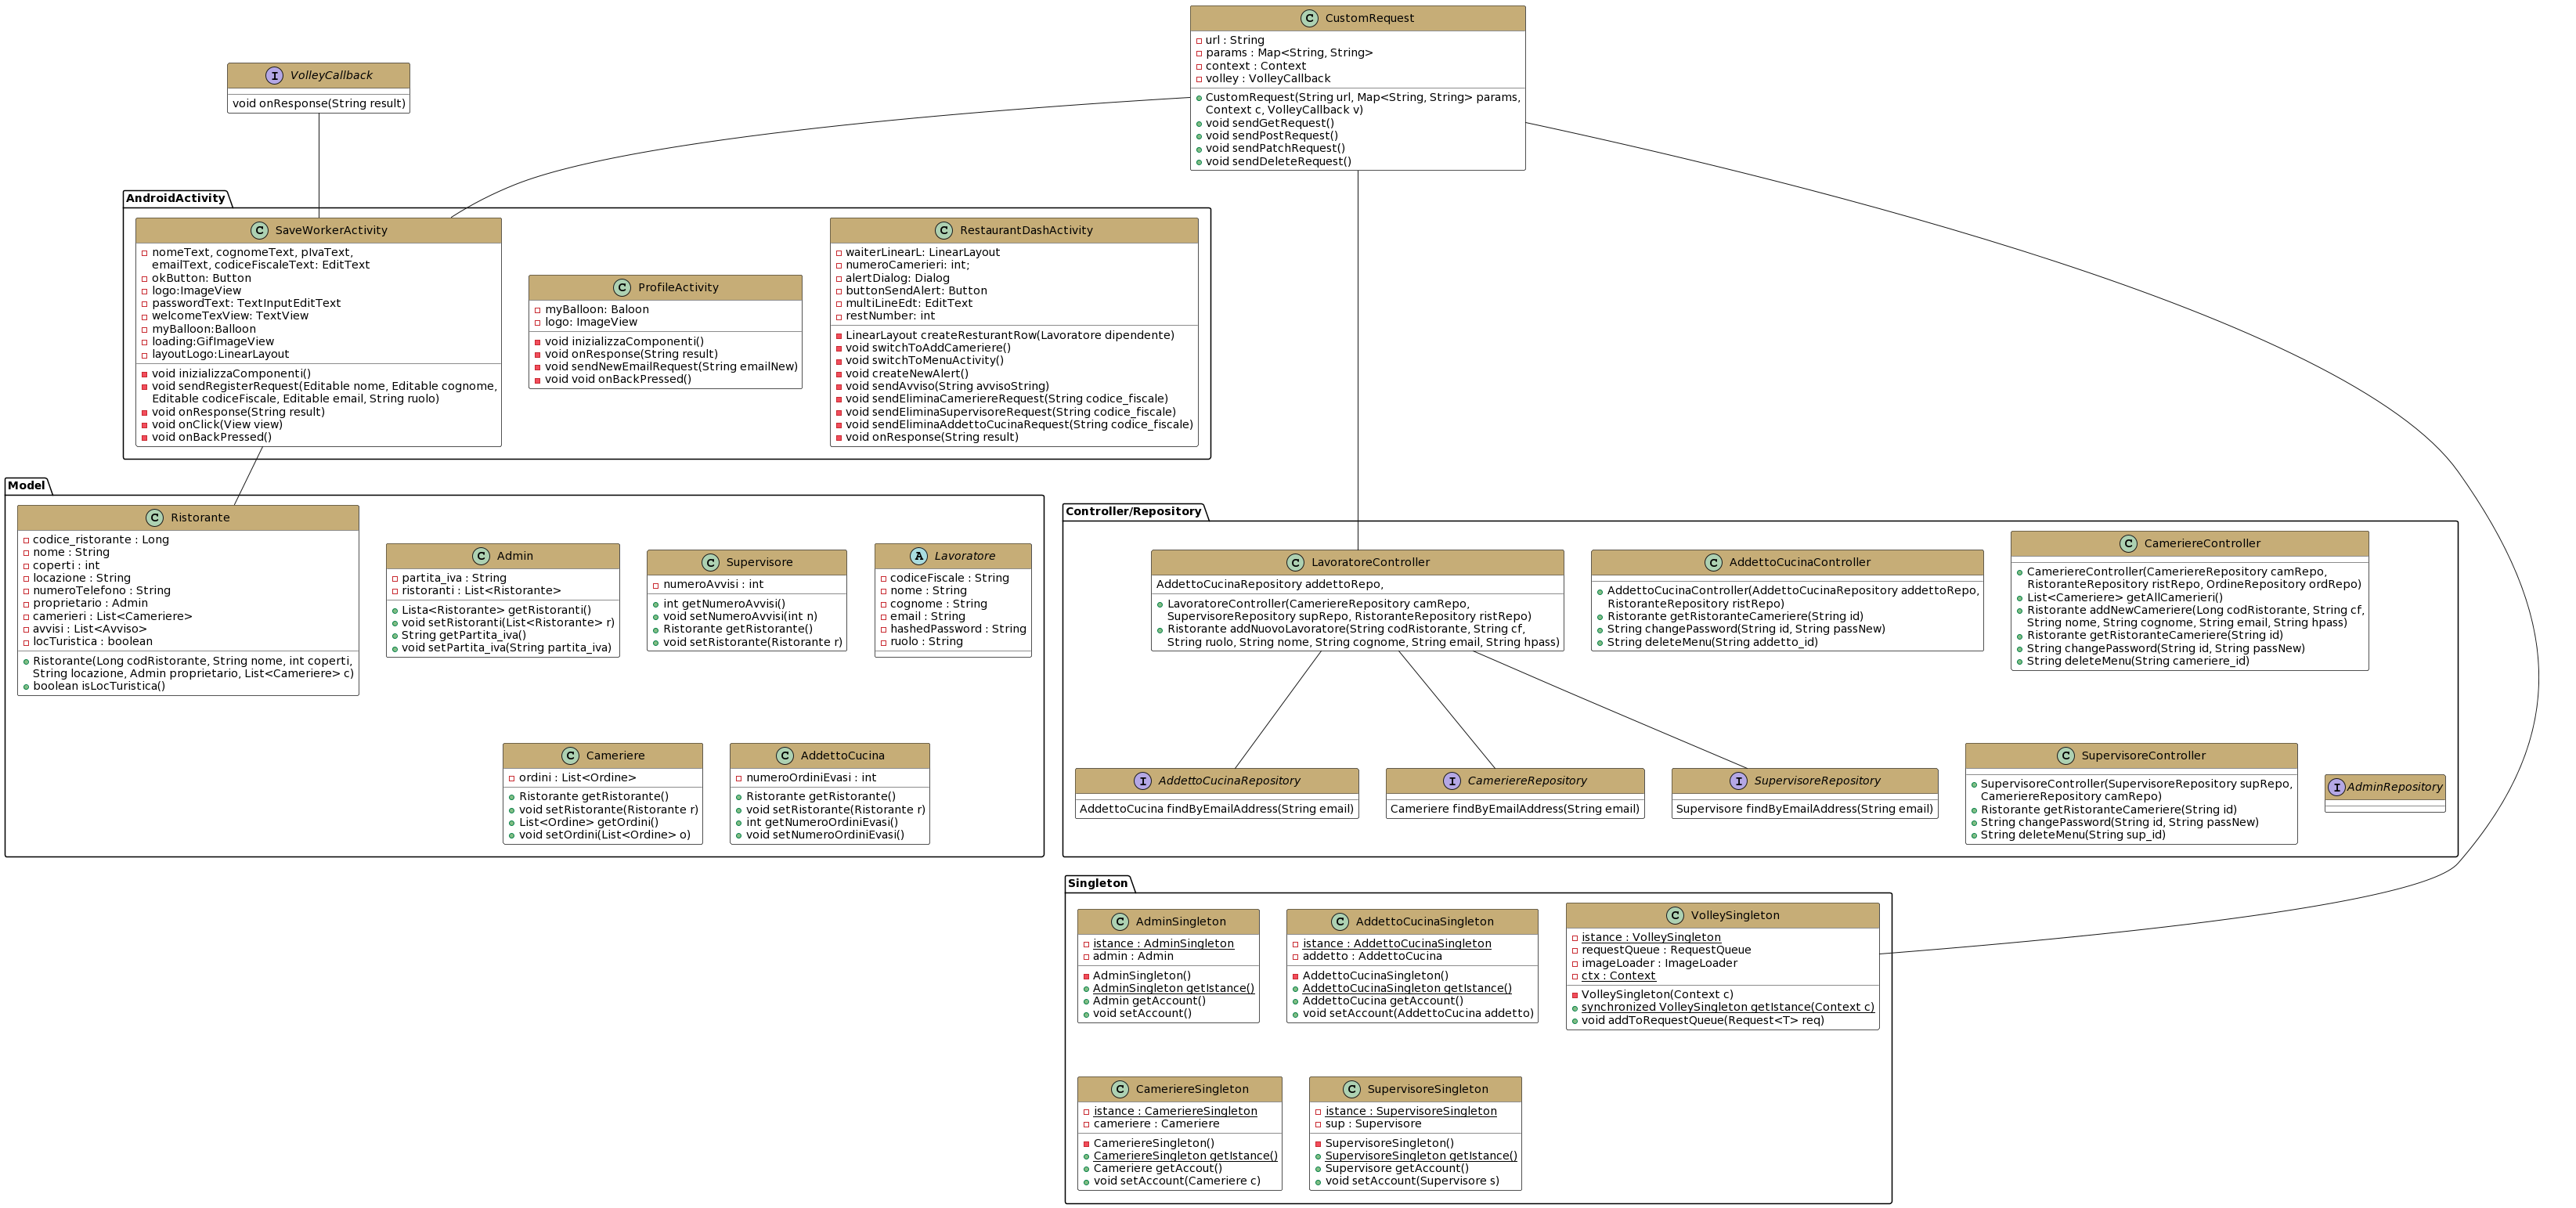
\includegraphics[scale=0.15]{assets/diagrammi/Class diagram di design/gestione dipendenti.png}
            \caption*{\textbf{CD03}: Class diagram gestione Dipdendenti}\label{fig:ClassDiagram_ManageWorkers}
        \end{figure}


